\subsubsection{Foam modeling}

\begin{wrapfigure}{l}{0.4\textwidth}
\vspace{-1em}
\centering
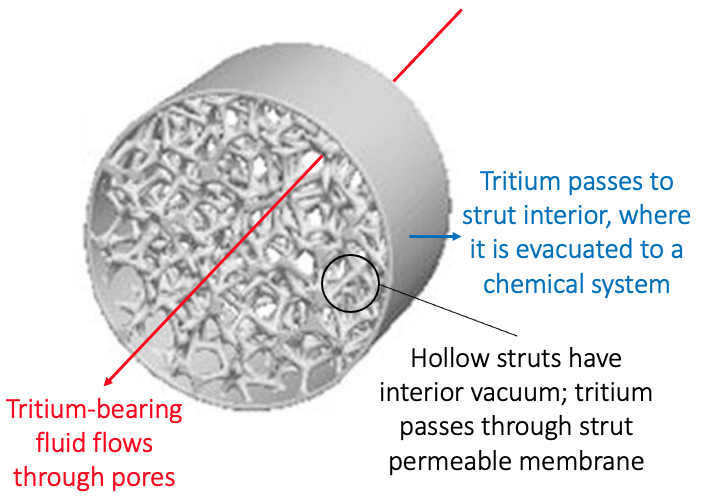
\includegraphics[width=.95\textwidth]{figs/foam.png}
 \caption{\label{fig:foam}\small Reticulated foam tritium extraction.\vspace{-1em}}
\end{wrapfigure}


. The tritium breeding ratio (TBR) is one of the most critical metrics in achieving viable fusion energy -- equally important is the ability for mass separations systems to then extract this generated tritium from a tritium-bearing transport fluid in a chemical plant. Today's extraction methods are largely based on decades-old tubular permeable membranes, which exhibit very high material cost and energy consumption needs \cite{abdou}. This INCITE renewal will perform 3-D simulations of tritium transport coupled to CFD for novel advanced manufacturing geometries being explored through a DOE-FES Early Career award \cite{taylor}. A challenge with advanced manufacturing designs is the large design space; Fig. \ref{fig:foam} shows a representation of a reticulated capillary foam consisting of a continuous network of interconnected ligaments which will be studied in this project. The high surface area facilitates high mass transfer of tritium, at expense of pressure losses. 

A detailed understanding of fluid flow through these foams is necessary to understand the boundary conditions on tritium mass transport (boundary transport may be a rate-limiting process). Enormous computing requirements are needed due to the extremely high surface area, as nearly the entire flow field must be meshed to high resolution. Such systems are not dissimilar to our team's expertise in pebble bed reactors \cite{min}. High computational cost has limited past simulations to idealized unit cells in ordered arrays \cite{boomsma,boomsma2}, which
are unrepresentative of the real physics due to their failure to capture the foam's inherent randomness \cite{habisreuther}.
Others use porous media methods with adaptations of
friction correlations developed for other systems (e.g. Ergun-type correlations for packed spheres). However, the strong relationship between pressure drop and the foam structure frequently exhibits discrepancies between simulation and experiment on the order of $\pm100$\% \cite{bracconi,edouard}, challenging our ability to optimize foam structures \cite{inayat}. The importance of improving tritium technologies has been emphasized in every recent national strategic guiding document. The National Academy of Sciences found that ``The scale and rate of tritium use, breeding and processing will be a major design feature and challenge of a D-T pilot'' \cite{nap}. Calls for fundamental R\&D on tritium extraction are widely emphasize in the fusion community \cite{cpfe,fesac}.

Our objectives for the next year are to develop datasets to illuminate two crucial questions:
\begin{enumerate}
\item Are reticulated foams a viable candidate for tritium extraction?
\item Can the modeling of these foams be simplified while still facilitating accurate exploration of the large advanced manufacturing design space?
\end{enumerate}

The tasks for the foam fluid flow simulations are:

\vspace{-.15in}
\begin{enumerate}[label=\textbf{\Roman*}]
\item \textbf{Develop robust meshing strategy} for CAD-generated foam structures based on small-scale domains and mesh refinement studies.
\item \textbf{LES simulation of 3 foams} (informed by experimental partners) for 10 values of Reynolds number. Extract pressure drop and compare against experimental data.
\end{enumerate}
\vspace{-.15in}
